\documentclass[11pt]{scrartcl}
\usepackage{evan}
\title{HW4}
\author{Dallin G and Evan L sawyer and alexander}
\date{3-5-2024}
\definecolor{palegreen}{rgb}{0.6, 0.98, 0.6}
\begin{document}
\maketitle
\begin{problem}[\textcolor{red}{Some (counter)-example}]\phantom{0}

    \begin{enumerate}[(i)]
        \item Give an example of a finite graded poset $P$ with the Sperner property, together with a group $G$ acting on $P$, such that $P/G$ is \textit{not} Sperner.
        \item Consider the poset $P$ whose Hasse diagram is given by
        \begin{center}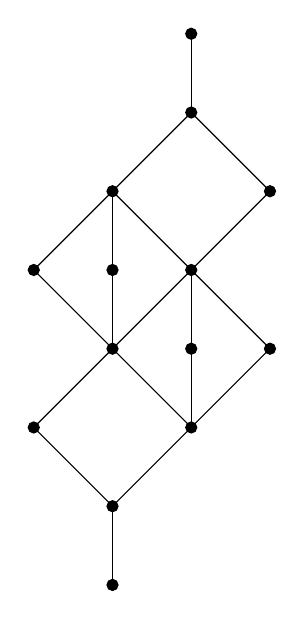
\begin{tikzpicture}
            \draw[fill=black] (0,-0.5) circle (2pt);
            \draw[fill=black] (0,0.5) circle (2pt);
            \draw[fill=black] (-1,1.5) circle (2pt);
            \draw[fill=black] (1,1.5) circle (2pt);
            \draw[fill=black] (0,2.5) circle (2pt);
            \draw[fill=black] (1,2.5) circle (2pt);
            \draw[fill=black] (2,2.5) circle (2pt);
            \draw[fill=black] (-1,3.5) circle (2pt);
            \draw[fill=black] (0,3.5) circle (2pt);
            \draw[fill=black] (1,3.5) circle (2pt);
            \draw[fill=black] (0,4.5) circle (2pt);
            \draw[fill=black] (2,4.5) circle (2pt);
            \draw[fill=black] (1,5.5) circle (2pt);
            \draw[fill=black] (1,6.5) circle (2pt);
            
            \draw (0,-0.5) -- (0,0.5);
            \draw (0,0.5 ) -- (-1,1.5);
            \draw (0,0.5) -- (1,1.5);
            \draw (1,1.5) -- (0,2.5);
            \draw (1,1.5) -- (1,2.5);
            \draw (1,1.5) -- (2,2.5);
            \draw (-1,1.5) -- (0,2.5);
            \draw (0,2.5) -- (-1,3.5);
            \draw (0,2.5) -- (0,3.5);
            \draw (0,2.5) -- (1,3.5);
            \draw (1,2.5) -- (1,3.5);
            \draw (2,2.5) -- (1,3.5);
            \draw (1,3.5) -- (0,4.5);
            \draw (1,3.5) -- (2,4.5);
            \draw (-1,3.5) -- (0,4.5);
            \draw (0,3.5) -- (0,4.5);
            \draw (0,4.5) -- (1,5.5);
            \draw (2,4.5) -- (1,5.5);
            \draw (1,5.5) -- (1,6.5);
            \end{tikzpicture}
            \end{center}
            Find a subgroup $G$ of $S_7$ such that $P\cong B_7/G$ or else prove that such a group does not exist.
    \end{enumerate}
\end{problem}
\begin{proof}[Proof (Dallin and Evan):]
    \begin{enumerate}[(i)]
        \item We draw a Hasse diagram for $P$:
        \begin{center}
            \begin{asy}
                size(4cm);
                pair A=(0,0),B=(1,0),C=(2,0),D=(3,0),E=(4,0),AA=(0,1),BB=(1,1),CC=(2,1),DD=(3,1),EE=(4,1);
                dot(A);dot(B);dot(C);dot(D);dot(E);dot(AA);dot(BB);dot(CC);dot(DD);dot(EE);
                draw(A--AA);draw(B--BB);draw(C--CC);draw(D--DD);draw(E--EE);
                label("$1$",AA,N);
                label("$2$",BB,N);
                label("$3$",CC,N);
                label("$4$",DD,N);
                label("$5$",EE,N);
                label("$6$",A,S);
                label("$7$",B,S);
                label("$8$",C,S);
                label("$9$",D,S);
                label("$10$",E,S);
            \end{asy}
        \end{center}
        We see that $P$ is Sperner by inspection; its largest antichain is of length four, and each rank has four elements. Let $G=((1, 2, 3), (8, 9, 10))$ be the group generated by the permutations $(1,2,3)$ and $(8,9,10)$. By drawing the Hasse diagram of $P/G$, we see that is clearly not Sperner:
        \begin{center}
            \begin{asy}
                size(4cm);
                pair A=(1,0),B=(2,0),C=(2,0),D=(3,0),BB=(2,1),CC=(2,1),DD=(3,1),EE=(4,1);
                dot(A);dot(C);dot(D);dot(BB);dot(CC);dot(DD);dot(EE);
                draw(A--BB);draw(C--BB);draw(D--CC);draw(D--DD);draw(D--EE);
                label("$1,2,3$",CC,N);
                label("$4$",DD,N);
                label("$5$",EE,N);
                label("$6$",A,S);
                label("$7$",B,S);
                label("$8,9,10$",D,S);
            \end{asy}
        \end{center}
        \item We claim that $B_n/G$ where $G$ is a group generated by permutations is isomorphic to $B_m$, where $m\leq n$. This result is since we effectively end up with the set of all subsets of $\{O_1,O_2,\dots\}$ where the $O_i$ are orbits in $\{1,2,\dots, n\}$ under the action of $G$. This will be isomorphic to $B_m$ under the mapping $O_m\to m$. However, the given poset has ranks of $1,1,2,3,3,2,1,1$, which are not the ranks of any boolean algebra.
    \end{enumerate}
\end{proof}
\begin{problem}[\textcolor{red}{Binary Necklace Poset}]
    A $(0,1)$-\textit{necklace} of \textit{length} $n$ and \textit{weight} $i$ is a circular arrangement of $i$ $1$'s and $n-i$ $0$'s. For instance, the $(0,1)$-necklaces of length $6$ and weight $3$ are (writing a circular arrangement linearly) $000111, 001011, 010011$ and $010101$. Cyclic shifts of a linear word represent the same necklace.

    \begin{enumerate}[(i)]
        \item (easy) Show that $N_n$ is rank-symmetric, rank-unimodal and Sperner.
    \end{enumerate}
\end{problem}
\begin{proof}[Proof (Dallin and Evan):]
    Notice that $N_n\cong B_n/G$, where $G$ is the group generated by the shift-by-one permutation $(1,2)(2,3),\dots,(n-1,n)$. This action also naturally preserves order, because order is strictly adding beads. Thus, by Theorem 5.8, $N_n$ is rank-symmetric, rank-unimodal, and Sperner.
\end{proof}
\begin{problem}
    Suppose $X$ is a finite set with $n$ elements. Let $G$ be a group of permutations on $X$. Thus $G$ acts on $2^X$. We say that $G$ acts \textit{transitively} on the $j$-element subsets if for every two $j$-element subsets $S$ and $T$, there is a $\pi\in G$ for which $\pi\cdot S=T$. Show that if $G$ acts transitively on $j$-element subsets for some $j\leq \frac n 2$, then $G$ acts transitively on $i$-element subsets for all $0\leq i\leq j$.
\end{problem}
\begin{proof}[Proof (Dallin and Evan):]
    We proceed by induction on $i$, with $G$ acting transitively on $i$-element subsets. Consider any two $i-1$-element subsets $S_1$ and $T_1$. Since $i\leq \frac{n}{2}$, we are guaranteed at least one element $a\in X$ not in $S_1$ or $T_1$. Define the function $\phi$ from the $i-1$ to the $i$-subsets of $X$ as the addition of $a$. Then, $\phi(S_1)$ and $\phi(T_1)$ are $i$-subsets, and by the inductive hypothesis, there is some $\pi\in G$ for which $\pi\cdot \phi(S_1)=\phi(T_1)$. Note that \[\pi(\phi(S_1))=\pi(S_1\cup\{a\})=T_1\cup\{a\},\] and since $\pi$ is a permutation, we must have $\pi\cdot S_1=T_1$. Thus, $G$ acts transitively on $i-1$-element subsets, and the induction is complete.
\end{proof}
\end{document}